\documentclass[11pt,letterpaper]{article}

% Packages
\usepackage{amsmath,amssymb,amsthm}
\usepackage{mathtools}
\usepackage{graphicx}
\usepackage{hyperref}
\usepackage{geometry}
\usepackage{booktabs}
\usepackage{tikz}
\usetikzlibrary{shapes,arrows,positioning}

\geometry{margin=1in}

% Theorem environments
\newtheorem{theorem}{Theorem}[section]
\newtheorem{lemma}[theorem]{Lemma}
\newtheorem{proposition}[theorem]{Proposition}
\newtheorem{corollary}[theorem]{Corollary}
\theoremstyle{definition}
\newtheorem{definition}[theorem]{Definition}
\newtheorem{example}[theorem]{Example}
\theoremstyle{remark}
\newtheorem{remark}[theorem]{Remark}

% Custom commands
\newcommand{\R}{\mathbb{R}}
\newcommand{\N}{\mathbb{N}}
\newcommand{\defeq}{\coloneqq}

\title{Stock-Flow Consistent Monetary Operations:\\
Sectoral Balances and the Refutation of Loanable Funds}
\author{Technical Documentation}
\date{\today}

\begin{document}

\maketitle

\begin{abstract}
We present a formal Stock-Flow Consistent (SFC) framework for understanding monetary operations in a modern fiat currency system. We derive the fundamental sectoral balance identity, demonstrate that bank credit creates deposits endogenously (horizontal money), show how fiscal operations inject net financial assets (vertical money), and prove that quantitative easing and bond operations are portfolio swaps that preserve private sector net wealth. This framework refutes the loanable funds doctrine by showing that credit is not constrained by prior savings. This document provides the theoretical foundation for an interactive web application that allows users to experiment with these operations and observe the balance sheet effects in real time.
\end{abstract}

\tableofcontents

\section{Introduction}

The loanable funds model treats savings as a prerequisite for investment, implying that banks are intermediaries between savers and borrowers. The Stock-Flow Consistent (SFC) framework, developed by Wynne Godley and refined by Modern Monetary Theory (MMT) economists including Warren Mosler and Stephanie Kelton, demonstrates that this view is fundamentally incorrect for modern monetary systems.

This document formalizes the accounting identities and operational mechanics that underpin an interactive Stock-Flow Consistent monetary laboratory. The web application implements these equations and allows users to post transactions and observe the resulting balance sheet changes across all four sectors simultaneously.

This document formalizes the key results:
\begin{itemize}
    \item The sectoral balance identity relating private and public net worth
    \item The mechanics of horizontal money (bank credit expansion)
    \item The mechanics of vertical money (fiscal operations)
    \item The nature of monetary operations (bonds, QE, QT)
    \item Balance sheet consistency across all sectors
\end{itemize}

\section{The Four-Sector Framework}

We model the economy using four consolidated balance sheets (see Figure \ref{fig:balance-sheets}):

\begin{definition}[The Four Sectors]
Let the economy consist of four sectors with balance sheets:
\begin{enumerate}
    \item \textbf{Treasury}: Assets $A_T$, Liabilities $L_T$, Net Worth $NW_T = A_T - L_T$
    \item \textbf{Central Bank (Fed)}: Assets $A_F$, Liabilities $L_F$, Net Worth $NW_F = A_F - L_F$
    \item \textbf{Banking System}: Assets $A_B$, Liabilities $L_B$, Net Worth $NW_B = A_B - L_B$
    \item \textbf{Households}: Assets $A_H$, Liabilities $L_H$, Net Worth $NW_H = A_H - L_H$
\end{enumerate}
\end{definition}

\subsection{Balance Sheet Components}

Let us define the key stock variables:
\begin{align}
D &\defeq \text{Bank deposits (household asset, bank liability)} \\
L &\defeq \text{Bank loans (bank asset, household liability)} \\
R &\defeq \text{Bank reserves (bank asset, Fed liability)} \\
B_H &\defeq \text{Treasury bonds held by households} \\
B_F &\defeq \text{Treasury bonds held by Fed} \\
\text{TGA} &\defeq \text{Treasury General Account (Treasury asset, Fed liability)}
\end{align}

% Figures for SFC monetary operations

\begin{figure}[htbp]
\centering
\renewcommand{\arraystretch}{1.25}
\setlength{\tabcolsep}{10pt}
\begin{tabular}{@{}lcccc@{}}
\toprule
 & \textbf{Households} & \textbf{Banks} & \textbf{Central bank} & \textbf{Treasury} \\
\midrule
Deposits $D$ & $+D$ & $-D$ &  &  \\
Loans $L$ & $-L$ & $+L$ &  &  \\
Reserves $R$ &  & $+R$ & $-R$ &  \\
Treasury securities & $+B_H$ &  & $+B_F$ & $-(B_H + B_F)$ \\
TGA ($\TGA$) &  &  & $-\TGA$ & $+\TGA$ \\
\bottomrule
\end{tabular}

\caption{Financial balance-sheet matrix (toy model). Positive entries are assets; negative entries are liabilities. Each row sums to zero across sectors. Private net financial assets are $R + B_H$.}
\label{fig:balance-sheets}
\end{figure}

\begin{figure}[htbp]
\centering
\resizebox{\textwidth}{!}{%
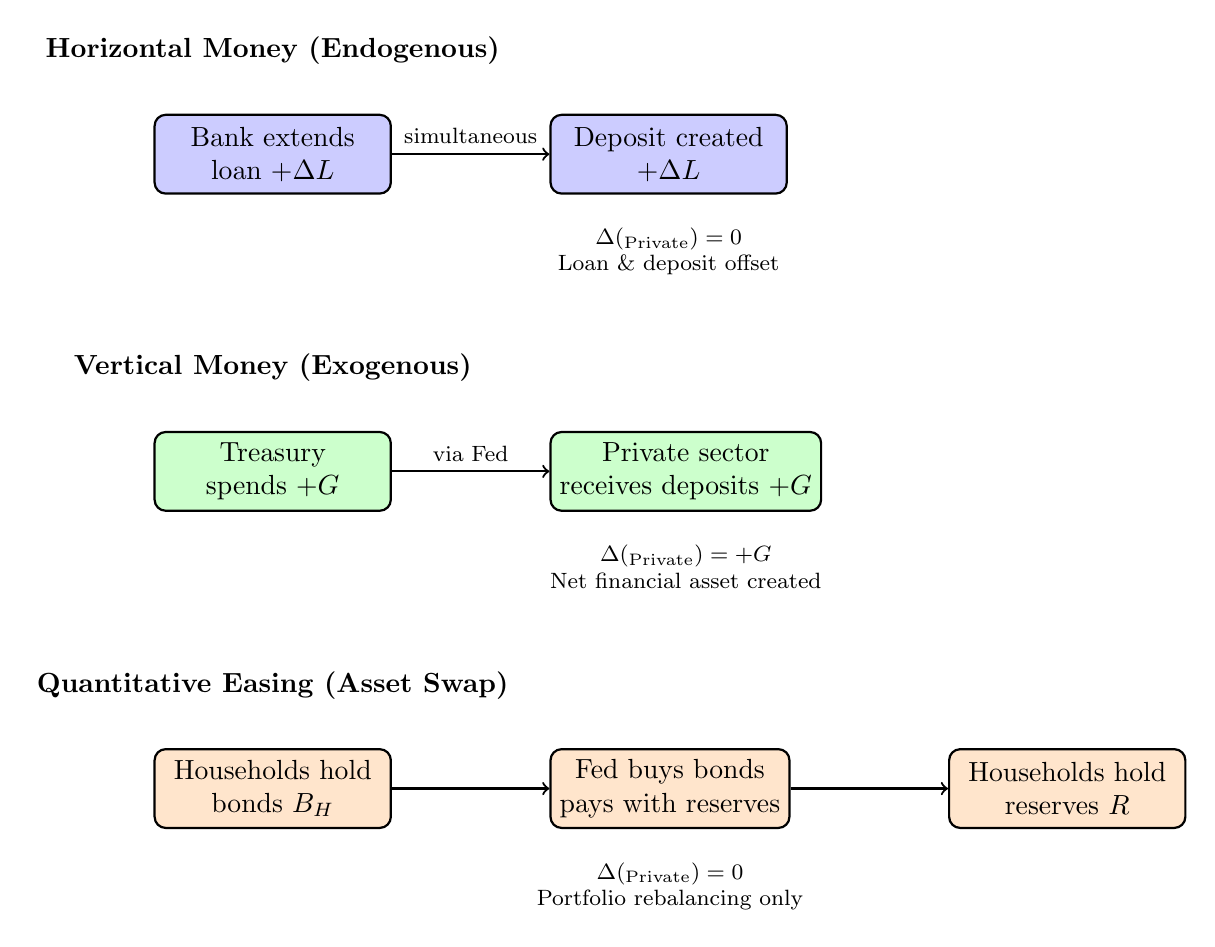
\begin{tikzpicture}[
    node distance=1.5cm and 2cm,
    process/.style={rectangle, rounded corners, draw=black, thick, minimum width=3cm, minimum height=1cm, align=center},
    flow/.style={->, thick},
    label/.style={font=\small}
]

% Horizontal Money Flow
\node[process, fill=blue!20] (bankloan) {Bank extends\\loan $+\Delta L$};
\node[process, fill=blue!20, right=of bankloan] (depositcreate) {Deposit created\\$+\Delta L$};
\node[label, above=0.5cm of bankloan, font=\bfseries] {Horizontal Money (Endogenous)};
\draw[flow] (bankloan) -- (depositcreate) node[midway, above, font=\footnotesize] {simultaneous};
\node[below=0.3cm of depositcreate, font=\footnotesize, align=center] {$\Delta(\NFA_{\text{Private}}) = 0$\\Loan \& deposit offset};

% Vertical Money Flow
\node[process, fill=green!20, below=3cm of bankloan] (treasury) {Treasury\\spends $+G$};
\node[process, fill=green!20, right=of treasury] (privatesector) {Private sector\\receives deposits $+G$};
\node[label, above=0.5cm of treasury, font=\bfseries] {Vertical Money (Exogenous)};
\draw[flow] (treasury) -- (privatesector) node[midway, above, font=\footnotesize] {via Fed};
\node[below=0.3cm of privatesector, font=\footnotesize, align=center] {$\Delta(\NFA_{\text{Private}}) = +G$\\Net financial asset created};

% QE Operation
\node[process, fill=orange!20, below=3cm of treasury] (qe1) {Households hold\\bonds $B_H$};
\node[process, fill=orange!20, right=of qe1] (qe2) {Fed buys bonds\\pays with reserves};
\node[process, fill=orange!20, right=of qe2] (qe3) {Households hold\\reserves $R$};
\node[label, above=0.5cm of qe1, font=\bfseries] {Quantitative Easing (Asset Swap)};
\draw[flow] (qe1) -- (qe2);
\draw[flow] (qe2) -- (qe3);
\node[below=0.3cm of qe2, font=\footnotesize, align=center] {$\Delta(\NFA_{\text{Private}}) = 0$\\Portfolio rebalancing only};

\end{tikzpicture}
}%
\caption{Three types of monetary operations. Horizontal money (bank lending) creates offsetting assets and liabilities. Vertical money (fiscal operations) changes private net financial assets. QE/QT are portfolio swaps that preserve private net financial assets.}
\label{fig:operations}
\end{figure}

% Multi-period dynamics figures
\begin{figure}[htbp]
\centering
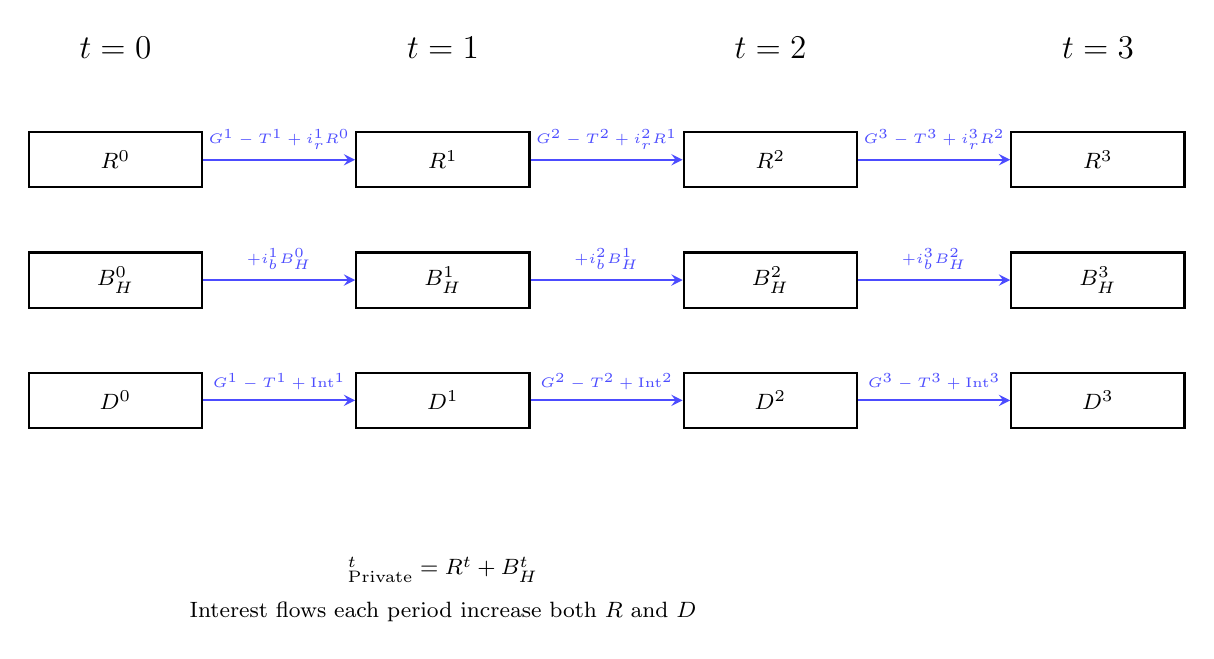
\begin{tikzpicture}[
    node distance=0.8cm and 3cm,
    stock/.style={rectangle, draw=black, thick, minimum width=2.2cm, minimum height=0.7cm, align=center, font=\footnotesize},
    flow/.style={->, thick, >=stealth},
    time/.style={font=\bfseries\large}
]

% Period t=0
\node[time] (t0) {$t=0$};
\node[stock, below=of t0] (r0) {$R^0$};
\node[stock, below=of r0] (bh0) {$B_H^0$};
\node[stock, below=of bh0] (d0) {$D^0$};

% Period t=1
\node[time, right=of t0] (t1) {$t=1$};
\node[stock, below=of t1] (r1) {$R^1$};
\node[stock, below=of r1] (bh1) {$B_H^1$};
\node[stock, below=of bh1] (d1) {$D^1$};

% Period t=2
\node[time, right=of t1] (t2) {$t=2$};
\node[stock, below=of t2] (r2) {$R^2$};
\node[stock, below=of r2] (bh2) {$B_H^2$};
\node[stock, below=of bh2] (d2) {$D^2$};

% Period t=3
\node[time, right=of t2] (t3) {$t=3$};
\node[stock, below=of t3] (r3) {$R^3$};
\node[stock, below=of r3] (bh3) {$B_H^3$};
\node[stock, below=of bh3] (d3) {$D^3$};

% Flow arrows with interest
\draw[flow, blue!70] (r0.east) -- (r1.west) node[midway, above, font=\tiny] {$G^1 - T^1 + i_r^1 R^0$};
\draw[flow, blue!70] (bh0.east) -- (bh1.west) node[midway, above, font=\tiny] {$+ i_b^1 B_H^0$};
\draw[flow, blue!70] (d0.east) -- (d1.west) node[midway, above, font=\tiny] {$G^1 - T^1 + \text{Int}^1$};

\draw[flow, blue!70] (r1.east) -- (r2.west) node[midway, above, font=\tiny] {$G^2 - T^2 + i_r^2 R^1$};
\draw[flow, blue!70] (bh1.east) -- (bh2.west) node[midway, above, font=\tiny] {$+ i_b^2 B_H^1$};
\draw[flow, blue!70] (d1.east) -- (d2.west) node[midway, above, font=\tiny] {$G^2 - T^2 + \text{Int}^2$};

\draw[flow, blue!70] (r2.east) -- (r3.west) node[midway, above, font=\tiny] {$G^3 - T^3 + i_r^3 R^2$};
\draw[flow, blue!70] (bh2.east) -- (bh3.west) node[midway, above, font=\tiny] {$+ i_b^3 B_H^2$};
\draw[flow, blue!70] (d2.east) -- (d3.west) node[midway, above, font=\tiny] {$G^3 - T^3 + \text{Int}^3$};

% NFA box
\node[below=1.5cm of d1, align=center, font=\footnotesize] (nfa) {
    $\NFA^t_{\text{Private}} = R^t + B_H^t$ \\[0.2cm]
    Interest flows each period increase both $R$ and $D$
};

\end{tikzpicture}
\caption{Multi-period stock evolution with interest payments. Each period, interest accrues on beginning-of-period stocks $(R^{t-1}, B_H^{t-1})$ and flows into reserves and deposits. Private net financial assets $\NFA^t = R^t + B_H^t$ grow by the nominal deficit.}
\label{fig:multiperiod-stocks}
\end{figure}

\begin{figure}[htbp]
\centering
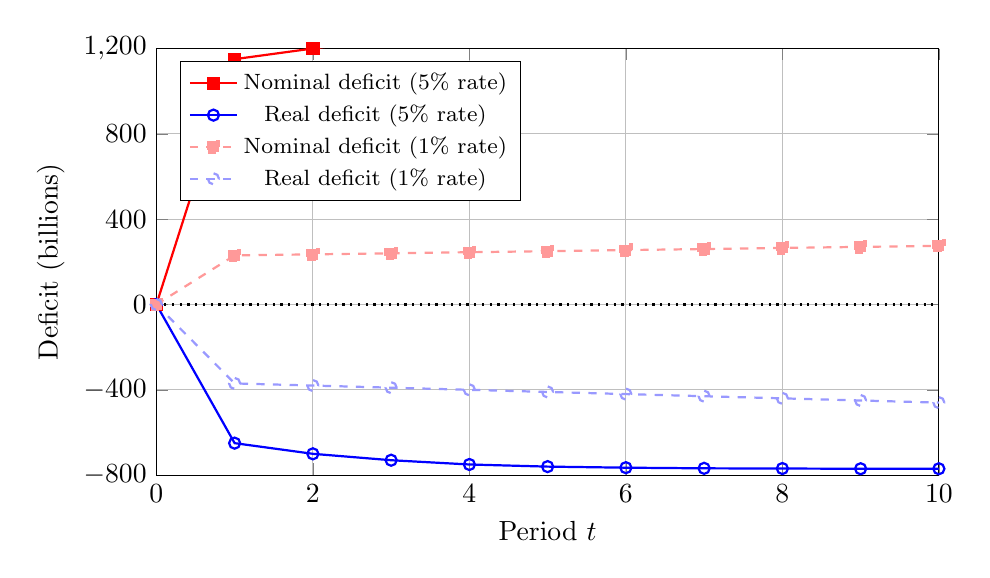
\begin{tikzpicture}
\begin{axis}[
    width=0.95\textwidth,
    height=7cm,
    xlabel={Period $t$},
    ylabel={Deficit (billions)},
    legend pos=north west,
    grid=major,
    xmin=0, xmax=10,
    ymin=-800, ymax=1200,
    xtick={0,2,4,6,8,10},
    ytick={-800,-400,0,400,800,1200},
    legend style={font=\footnotesize},
    every axis plot/.append style={thick}
]

% Nominal deficit - rate hike scenario (5% rate)
\addplot[color=red, mark=square*] coordinates {
    (0,0) (1,1150) (2,1200) (3,1250) (4,1300) (5,1350) (6,1400) (7,1450) (8,1500) (9,1550) (10,1600)
};
\addlegendentry{Nominal deficit (5\% rate)}

% Real deficit - rate hike scenario
\addplot[color=blue, mark=o] coordinates {
    (0,0) (1,-650) (2,-700) (3,-730) (4,-750) (5,-760) (6,-765) (7,-768) (8,-769) (9,-770) (10,-770)
};
\addlegendentry{Real deficit (5\% rate)}

% Nominal deficit - low rate scenario (1% rate)
\addplot[color=red!40, mark=square*, dashed] coordinates {
    (0,0) (1,230) (2,235) (3,240) (4,245) (5,250) (6,255) (7,260) (8,265) (9,270) (10,275)
};
\addlegendentry{Nominal deficit (1\% rate)}

% Real deficit - low rate scenario
\addplot[color=blue!40, mark=o, dashed] coordinates {
    (0,0) (1,-370) (2,-380) (3,-390) (4,-400) (5,-410) (6,-420) (7,-430) (8,-440) (9,-450) (10,-460)
};
\addlegendentry{Real deficit (1\% rate)}

\draw[dotted, thick] (axis cs:0,0) -- (axis cs:10,0);

\end{axis}
\end{tikzpicture}
\caption{Multi-period nominal vs.\ real deficit trajectories under high-debt scenario (120\% debt/GDP). Rate hike from 1\% to 5\% increases nominal deficit sharply (via interest payments) but produces \emph{larger real surplus} due to inflation erosion. Illustrates Mosler's deficit channel: rate hikes can be inflationary when debt is high.}
\label{fig:deficit-trajectories}
\end{figure}


\section{The Fundamental Sectoral Balance Identity}

\begin{theorem}[Sectoral Balance Identity]
\label{thm:sectoral-balance}
The private sector's net financial wealth equals the negative of the consolidated public sector's net worth:
\[
\text{Private NFW} = -(NW_T + NW_F)
\]
where Private Net Financial Wealth (NFW) is defined as:
\[
\text{Private NFW} = R + B_H
\]
\end{theorem}

\begin{proof}
We construct the balance sheets for each sector and derive the identity.

\textbf{Treasury Balance Sheet:}
\begin{align}
A_T &= \text{TGA} \\
L_T &= B_H + B_F \\
NW_T &= \text{TGA} - (B_H + B_F)
\end{align}

\textbf{Federal Reserve Balance Sheet:}
\begin{align}
A_F &= B_F \\
L_F &= R + \text{TGA} \\
NW_F &= B_F - R - \text{TGA}
\end{align}

\textbf{Consolidated Public Sector:}
\begin{align}
NW_{\text{Public}} &= NW_T + NW_F \\
&= (\text{TGA} - B_H - B_F) + (B_F - R - \text{TGA}) \\
&= -B_H - R
\end{align}

\textbf{Private Net Financial Wealth:}
The private sector holds reserves $R$ and bonds $B_H$ as financial assets (netting out loans and deposits which cancel):
\[
\text{Private NFW} = R + B_H = -(NW_T + NW_F)
\]
\end{proof}

\begin{remark}
This identity is an accounting identity, not a behavioral relationship. It holds by construction in a closed economy with consolidated sectors.
\end{remark}

\section{Horizontal Money: Endogenous Credit Creation}

See Figure \ref{fig:operations} for a visualization of the three types of monetary operations.

\begin{definition}[Horizontal Money]
Horizontal money refers to money created through bank lending. It expands both assets and liabilities on bank and household balance sheets simultaneously.
\end{definition}

\begin{proposition}[Bank Credit Expansion]
\label{prop:credit-expansion}
When a bank extends credit of amount $\Delta L > 0$:
\begin{enumerate}
    \item Bank assets increase by $\Delta L$ (new loan)
    \item Bank liabilities increase by $\Delta L$ (new deposit)
    \item Household assets increase by $\Delta L$ (new deposit)
    \item Household liabilities increase by $\Delta L$ (new loan)
    \item Private Net Financial Wealth is unchanged: $\Delta(\text{Private NFW}) = 0$
    \item Public sector net worth is unchanged: $\Delta(NW_{\text{Public}}) = 0$
\end{enumerate}
\end{proposition}

\begin{proof}
The double-entry bookkeeping entries are:

\textbf{Bank:}
\begin{itemize}
    \item Debit: Loans $+\Delta L$
    \item Credit: Deposits $+\Delta L$
\end{itemize}

\textbf{Household:}
\begin{itemize}
    \item Debit: Deposits $+\Delta L$
    \item Credit: Loans $+\Delta L$
\end{itemize}

Bank equity: $NW_B = (A_B + \Delta L) - (L_B + \Delta L) = NW_B$ (unchanged)

Household net worth: $NW_H = (A_H + \Delta L) - (L_H + \Delta L) = NW_H$ (unchanged)

Private NFW consists of reserves and bonds, neither of which changed, so $\Delta(\text{Private NFW}) = 0$.
\end{proof}

\begin{corollary}[Refutation of Loanable Funds - Part I]
Bank lending does not require prior savings. Deposits are created simultaneously with loans.
\end{corollary}

\section{Vertical Money: Fiscal Operations}

\begin{definition}[Vertical Money]
Vertical money refers to money created through government fiscal operations (spending and taxation). It changes the net financial assets held by the private sector.
\end{definition}

\subsection{Fiscal Spending}

\begin{proposition}[Fiscal Spending]
\label{prop:fiscal-spending}
When the Treasury spends amount $G > 0$:
\begin{enumerate}
    \item Treasury's TGA decreases by $G$
    \item Bank reserves increase by $G$
    \item Household deposits increase by $G$
    \item Private Net Financial Wealth increases by $G$
    \item Public sector net worth decreases by $G$
\end{enumerate}
\end{proposition}

\begin{proof}
The double-entry operations:

\textbf{Treasury:}
\begin{itemize}
    \item Credit: TGA $-G$
\end{itemize}

\textbf{Federal Reserve:}
\begin{itemize}
    \item Debit: Reserves $+G$
    \item Credit: TGA $-G$
\end{itemize}

\textbf{Banking System:}
\begin{itemize}
    \item Debit: Reserves $+G$
    \item Credit: Deposits $+G$
\end{itemize}

\textbf{Households:}
\begin{itemize}
    \item Debit: Deposits $+G$
\end{itemize}

Changes to sectoral net worth:
\begin{align}
\Delta NW_T &= -G \\
\Delta NW_F &= 0 \quad \text{(both assets and liabilities increased by } G) \\
\Delta(\text{Private NFW}) &= +G \quad \text{(reserves increased)}
\end{align}

Verifying the identity: $\Delta(\text{Private NFW}) = -\Delta(NW_T + NW_F) = -(-G + 0) = +G$ $\checkmark$
\end{proof}

\subsection{Taxation}

\begin{proposition}[Taxation]
Taxation is the inverse of spending. When taxes $T > 0$ are collected:
\begin{enumerate}
    \item Private Net Financial Wealth decreases by $T$
    \item Public sector net worth increases by $T$
\end{enumerate}
\end{proposition}

\begin{corollary}[Fiscal Deficits Create Net Financial Assets]
A fiscal deficit $(G - T) > 0$ increases private sector net financial wealth by exactly $(G - T)$.
\end{corollary}

\section{Monetary Operations: Portfolio Swaps}

\subsection{Bond Issuance}

\begin{proposition}[Bond Issuance]
When the Treasury issues bonds $B$ to the private sector:
\begin{enumerate}
    \item Household deposits decrease by $B$
    \item Household bond holdings increase by $B$
    \item Bank reserves decrease by $B$
    \item Treasury's TGA increases by $B$
    \item Private Net Financial Wealth is unchanged
\end{enumerate}
\end{proposition}

\begin{proof}
This is an asset swap for households: reserves $\to$ bonds.

Private NFW before: $R + B_H$

Private NFW after: $(R - B) + (B_H + B) = R + B_H$

Therefore $\Delta(\text{Private NFW}) = 0$.
\end{proof}

\subsection{Quantitative Easing (QE)}

\begin{proposition}[Quantitative Easing]
When the Fed purchases bonds $Q$ from the private sector:
\begin{enumerate}
    \item Household bond holdings decrease by $Q$
    \item Fed bond holdings increase by $Q$
    \item Household deposits increase by $Q$
    \item Bank reserves increase by $Q$
    \item Private Net Financial Wealth is unchanged
\end{enumerate}
\end{proposition}

\begin{proof}
Another asset swap for households: bonds $\to$ reserves.

Private NFW before: $R + B_H$

Private NFW after: $(R + Q) + (B_H - Q) = R + B_H$

Therefore $\Delta(\text{Private NFW}) = 0$.
\end{proof}

\begin{remark}
QE and QT (Quantitative Tightening, the reverse operation) are portfolio rebalancing operations. They do not change the private sector's net financial wealth, only its composition.
\end{remark}

\section{Balance Sheet Integrity}

We can verify that all four balance sheets remain balanced after each operation:

\begin{theorem}[Balance Sheet Consistency]
For each sector $i \in \{T, F, B, H\}$, the accounting identity $A_i = L_i + NW_i$ holds before and after any monetary operation.
\end{theorem}

\section{Implications and Conclusion}

\subsection{Refutation of Loanable Funds}

The loanable funds doctrine asserts that:
\begin{enumerate}
    \item Banks lend out savings (FALSE: Proposition \ref{prop:credit-expansion})
    \item Government deficits crowd out private investment (FALSE: Proposition \ref{prop:fiscal-spending})
    \item Central bank operations change money supply (MISLEADING: they change composition, not net wealth)
\end{enumerate}

The SFC framework shows:
\begin{itemize}
    \item Banks create deposits when they lend (endogenous money)
    \item Fiscal deficits create the net financial assets the private sector desires
    \item QE/QT swap asset types without changing private wealth
\end{itemize}

\subsection{Policy Implications}

\begin{enumerate}
    \item The binding constraint on bank lending is not deposits but creditworthy borrowers and capital requirements
    \item Government deficits are necessary to provide net financial assets to the private sector when the private sector desires to net save
    \item Interest rate changes via QE/QT work through portfolio rebalancing effects, not changes in the quantity of money
    \item The Treasury General Account (TGA) target mechanism shown in the interactive application demonstrates how bond issuance coordinates with fiscal operations to maintain desired government deposit levels
\end{enumerate}

\subsection{Interactive Application}

The accompanying web application (\texttt{src/App.jsx}) implements these operations with the following features:
\begin{itemize}
    \item Real-time balance sheet updates across all four sectors
    \item Automatic TGA targeting via bond issuance/redemption
    \item Visual verification of the sectoral balance identity: Private NFW + Public NW = 0
    \item Constraints that prevent operations from creating negative stocks (e.g., cannot tax more than existing deposits)
\end{itemize}

Users can experiment with different magnitudes of fiscal spending, taxation, bank lending, and monetary operations to develop intuition for how these transactions flow through the consolidated sectoral accounts.

\section{References}

\begin{itemize}
    \item Godley, W., \& Lavoie, M. (2007). \textit{Monetary Economics: An Integrated Approach to Credit, Money, Income, Production and Wealth}. Palgrave Macmillan.
    \item Mosler, W. (1993--2010). \textit{Soft Currency Economics} and related papers.
    \item Kelton, S. (2020). \textit{The Deficit Myth: Modern Monetary Theory and the Birth of the People's Economy}. PublicAffairs.
    \item Keen, S. (2011). \textit{Debunking Economics: The Naked Emperor Dethroned?} Zed Books.
\end{itemize}

\end{document}
